%% ============================================================
%%  PRAXIS — Whitepaper
%%  Goal-Aligned Social Operating System
%% ============================================================
\documentclass[11pt,a4paper]{article}

% ── Packages ──────────────────────────────────────────────
\usepackage[margin=2.5cm]{geometry}
\setlength{\headheight}{22pt}
\addtolength{\topmargin}{-10pt}
\usepackage[T1]{fontenc}
\usepackage[utf8]{inputenc}
\usepackage{lmodern}
\usepackage{microtype}
\usepackage{xcolor}
\usepackage{graphicx}
\usepackage{amsmath,amssymb}
\usepackage{booktabs}
\usepackage{tabularx}
\usepackage{longtable}
\usepackage{multirow}
\usepackage{array}
\usepackage{enumitem}
\usepackage{hyperref}
\usepackage{fancyhdr}
\usepackage{titlesec}
\usepackage{abstract}
\usepackage{setspace}
\usepackage{caption}
\usepackage{subcaption}
\usepackage{tcolorbox}
\usepackage{fontawesome5}
\usepackage{tikz}
\usepackage{pgfplots}
\pgfplotsset{compat=1.18}
\usetikzlibrary{positioning,shapes.geometric,arrows.meta,calc,backgrounds,fit}

% ── Colours ───────────────────────────────────────────────
\definecolor{amber}{HTML}{F59E0B}
\definecolor{amberlight}{HTML}{FDE68A}
\definecolor{amberdark}{HTML}{B45309}
\definecolor{violet}{HTML}{7C3AED}
\definecolor{violetlight}{HTML}{DDD6FE}
\definecolor{darkbg}{HTML}{0F0F0F}
\definecolor{midgray}{HTML}{374151}
\definecolor{lightgray}{HTML}{F3F4F6}
\definecolor{successgreen}{HTML}{10B981}
\definecolor{linkblue}{HTML}{2563EB}

% ── Hyperref setup ────────────────────────────────────────
\hypersetup{
  colorlinks=true,
  linkcolor=amberdark,
  citecolor=amberdark,
  urlcolor=linkblue,
  pdftitle={Praxis — Whitepaper},
  pdfauthor={Praxis Technologies},
  pdfsubject={Goal-Aligned Social Operating System},
  pdfkeywords={goal-alignment, social network, accountability, AI matching, peer verification}
}

% ── Header / Footer ───────────────────────────────────────
\pagestyle{fancy}
\fancyhf{}
\fancyhead[L]{\small\textcolor{midgray}{\textsc{Praxis} — Confidential Whitepaper}}
\fancyhead[R]{\small\textcolor{midgray}{Version 1.0 · February 2026}}
\fancyfoot[C]{\small\textcolor{midgray}{\thepage}}
\renewcommand{\headrulewidth}{0.4pt}
\renewcommand{\headrule}{\hbox to\headwidth{\color{amber}\leaders\hrule height \headrulewidth\hfill}}

% ── Section styles ────────────────────────────────────────
\titleformat{\section}
  {\large\bfseries\color{amberdark}}
  {\thesection.}{0.75em}{}[\vspace{-4pt}\color{amber}\rule{\linewidth}{1.5pt}]

\titleformat{\subsection}
  {\normalsize\bfseries\color{midgray}}
  {\thesubsection.}{0.5em}{}

\titleformat{\subsubsection}
  {\normalsize\itshape\color{midgray}}
  {\thesubsubsection.}{0.5em}{}

% ── tcolorbox styles ──────────────────────────────────────
\tcbuselibrary{skins,breakable}

\newtcolorbox{calloutbox}[2][]{
  enhanced, breakable,
  colback=amberlight!30, colframe=amber,
  fonttitle=\bfseries\color{amberdark},
  title={#2}, #1,
  left=6pt, right=6pt, top=4pt, bottom=4pt
}

\newtcolorbox{statbox}[1][]{
  enhanced, breakable,
  colback=lightgray, colframe=midgray!40,
  left=6pt, right=6pt, top=4pt, bottom=4pt,
  #1
}

\newtcolorbox{pitchbox}{
  enhanced, breakable,
  colback=darkbg, colframe=amber,
  coltitle=amber, fonttitle=\large\bfseries,
  title={\faRocket\quad The Praxis Opportunity},
  coltext=white,
  left=10pt, right=10pt, top=8pt, bottom=8pt
}

% ── Misc ──────────────────────────────────────────────────
\setlength{\parskip}{5pt}
\setlength{\parindent}{0pt}
\captionsetup{font=small,labelfont={bf,color=midgray}}

% ─────────────────────────────────────────────────────────
\begin{document}

% ══════════════════════════════════════════════════════════
%  TITLE PAGE
% ══════════════════════════════════════════════════════════
\begin{titlepage}
\pagecolor{darkbg}
\color{white}

\begin{center}
\vspace*{2cm}

% Logo / wordmark
{\fontsize{64}{72}\selectfont\textbf{\textcolor{amber}{P}}\textcolor{white}{raxis}}

\vspace{0.4cm}
{\large\textcolor{amberlight}{\textit{Goal-Aligned Social Operating System}}}

\vspace{0.8cm}
\textcolor{amber}{\rule{10cm}{1pt}}

\vspace{1.2cm}
{\LARGE\bfseries Technical \& Investment Whitepaper}

\vspace{0.6cm}
{\normalsize Version 1.0 \quad|\quad February 2026 \quad|\quad Private \& Confidential}

\vspace{2.5cm}

% Tagline box
\fcolorbox{amber}{darkbg}{%
  \parbox{12cm}{%
    \centering
    \vspace{0.5cm}
    {\large\textcolor{amberlight}{\textit{``Goals unite us. Rigor guides us. Collaboration transforms us.''}}}
    \vspace{0.5cm}
  }%
}

\vspace{3cm}

\begin{tabular}{ccc}
\textcolor{amber}{\Large\faUsers} &\quad\quad& \textcolor{amber}{\Large\faBullseye} \\[4pt]
\textcolor{amberlight}{Community-Driven} && \textcolor{amberlight}{Goal-Focused} \\[16pt]
\textcolor{amber}{\Large\faBrain} &\quad\quad& \textcolor{amber}{\Large\faMedal} \\[4pt]
\textcolor{amberlight}{AI-Powered Matching} && \textcolor{amberlight}{Peer-Verified Progress}
\end{tabular}

\vfill

{\small\textcolor{midgray}{%
  Praxis Technologies · \href{mailto:contact@praxis.app}{contact@praxis.app}\\
  This document is intended for authorised recipients only.
  Redistribution without written consent is prohibited.
}}
\end{center}
\end{titlepage}

\nopagecolor   % reset background after title

% ══════════════════════════════════════════════════════════
%  TABLE OF CONTENTS
% ══════════════════════════════════════════════════════════
\newpage
\tableofcontents

% ══════════════════════════════════════════════════════════
%  ABSTRACT
% ══════════════════════════════════════════════════════════
\newpage
\begin{abstract}
\noindent
Praxis is a \textbf{goal-aligned social operating system} that connects individuals based on shared ambitions, compatible progress trajectories, and mutual accountability commitments — not appearance, demographics, or superficial interest tags. In an era characterised simultaneously by a \textit{global loneliness epidemic} and an explosion in personal-development spending, existing platforms fail the user at the precise moment of execution: they either optimise for engagement over outcomes (social networks), for appearance over values (dating apps), or for shallow connection over deep collaboration (professional networks).

Praxis addresses this gap through three interlocking innovations: (1)~a \textbf{multi-domain hierarchical goal tree} that encodes a user's full ambition profile across nine life domains; (2)~an \textbf{AI-powered semantic matching engine} using Gemini embeddings and cosine-similarity scoring to identify the most compatible accountability partner from the entire user base; and (3)~a \textbf{peer verification protocol} that makes progress claims socially credible and auto-triggers community recognition.

The platform currently operates as a production-grade MVP, deployed on a modern stack (React / TypeScript / Express / Supabase / pgvector), with a freemium subscription model and a novel \textbf{accountability betting} mechanism for premium users. This whitepaper presents the product rationale, the mathematical underpinnings of the matching algorithm, the competitive landscape, and a detailed financial thesis.

\bigskip
\noindent\textbf{Keywords:} goal-alignment, accountability, peer verification, AI matching, social operating system, pgvector, semantic embeddings, freemium, personal development.
\end{abstract}

% ══════════════════════════════════════════════════════════
%  1. THE PROBLEM
% ══════════════════════════════════════════════════════════
\newpage
\section{The Problem: Ambition Without Infrastructure}

\subsection{The Achievement Gap}

Humans are extraordinary at articulating ambitions. They are, statistically, poor at achieving them.

\begin{statbox}
\begin{itemize}[nosep]
  \item \textbf{91\%} of people fail to achieve their New Year's resolutions \\ {\small (University of Scranton; \textit{Inc.} Magazine)}
  \item \textbf{January 19} — ``Quitter's Day'' — is the statistically most common date resolutions are abandoned \\ {\small (Strava, analysis of 800~million logged activities)}
  \item Only \textbf{19\%} of goal-setters maintain progress two years after setting a goal \\ {\small (Discovery Happy Habits)}
\end{itemize}
\end{statbox}

This is not a motivation problem. Research consistently demonstrates that the single most effective lever for goal achievement is \textit{social accountability}:

\begin{calloutbox}{Research Finding — Dominican University of California}
Dr.~Gail Matthews found that individuals who \textbf{wrote down their goals and shared weekly updates with an accountability partner achieved a 76\% success rate}, compared to 43\% for those who simply thought about their goals — a~\textbf{77\% relative improvement}.

The American Society of Training and Development (ASTD) corroborates this: people are \textbf{65\%} more likely to achieve a goal after committing to another person, and \textbf{95\%} likely when ongoing check-in meetings are scheduled.
\end{calloutbox}

The infrastructure to systematically connect goal-aligned individuals does not yet exist at scale. This is the market Praxis enters.

\subsection{The Loneliness Paradox}

Modern connectivity has paradoxically intensified social isolation. Despite carrying supercomputers that connect us to billions of people, a record proportion of the population reports feeling profoundly alone.

\begin{statbox}
\begin{itemize}[nosep]
  \item \textbf{20\%} of U.S.\ adults experience loneliness \textit{daily} — up from 18\% the prior year \\ {\small (Gallup, August–September 2024)}
  \item \textbf{1 in 3} Americans feels lonely at least once a week \\ {\small (American Psychiatric Association Poll)}
  \item Chronic loneliness increases the risk of \textbf{premature death} equivalently to smoking 15 cigarettes per day and raises cardiovascular disease risk by~29\% \\ {\small (U.S.\ Surgeon General Advisory, May 2023)}
  \item Adults aged \textbf{30–44} are the loneliest demographic cohort, with~29\% reporting frequent or constant loneliness \\ {\small (Science of People, 2026, citing 2024 Surgeon General data)}
  \item \textbf{81\%} of lonely adults report co-occurring anxiety or depression, vs.\ 29\% of connected adults \\ {\small (Harvard Making Caring Common, 2024)}
\end{itemize}
\end{statbox}

Loneliness is not the absence of people; it is the absence of \textit{meaningful} connection. Praxis is engineered for the latter.

\subsection{Platform Failures}

\subsubsection{Social Networks (Instagram, TikTok, X)}
Optimised for engagement and advertisement revenue. Algorithmic feeds reward outrage, comparison, and performative living. The outcome for users: higher anxiety, lower self-esteem, and no progress on actual goals.

\subsubsection{Dating Apps}
\begin{statbox}
\begin{itemize}[nosep]
  \item \textbf{78\%} of users feel emotionally exhausted by online dating; \textbf{79\%} of Gen~Z/Millennial users report ``dating app burnout'' \\ {\small (Forbes Health Survey, 2024, $n=1{,}000$)}
  \item \textbf{46\%} of current users describe their experience as \textit{bad} \\ {\small (UK nationally representative poll, 2024)}
  \item Dating app users are \textbf{less satisfied with their relationship status} than non-users \\ {\small (Radboud University, \textit{phys.org}, February 2024)}
  \item Male match rates on Tinder average \textbf{below 5\%}, with some analyses reporting as low as~0.6\%
\end{itemize}
\end{statbox}

These platforms match on appearance. Praxis matches on aspiration.

\subsubsection{Professional Networks (LinkedIn)}
LinkedIn's \textbf{1.2 billion registered users} and \textbf{310 million monthly actives} generate a paradox: the average user maintains $\approx$1,300 connections yet struggles to identify even a handful of people actively building similar skills or pursuing similar professional outcomes. Volume displaces depth.

\subsubsection{Accountability Apps (Focusmate, Habitica, Coach.me)}
These tools address specific productivity niches — body-doubling for focus sessions, gamified habit streaks — but none offers \textit{semantic} goal alignment, holistic multi-domain identity, verified completion, or a scalable real-time communication layer. They are point solutions; Praxis is an operating system.

% ══════════════════════════════════════════════════════════
%  2. MARKET OPPORTUNITY
% ══════════════════════════════════════════════════════════
\section{Market Opportunity}

\subsection{Total Addressable Market (TAM)}

Praxis operates at the intersection of four large and growing markets:

\begin{center}
\begin{tabular}{lrrl}
\toprule
\textbf{Segment} & \textbf{2024 Value} & \textbf{Projected} & \textbf{CAGR} \\
\midrule
Global Wellness Economy & \$6.8T & \$9.8T (2029) & 7.6\% \\
Personal Development Market & \$38.4B & \$57.1B (2032) & 5.2\% \\
Self-Improvement Market & \$45.7B & \$84.0B (2034) & 6.3\% \\
Habit Tracking App Market & \$11.4B & \$43.9B (2034) & 14.4\% \\
Life Coaching Market & \$3.6B & \$6.1B (2031) & 9.1\% \\
AI Companion / Social AI & \$14.1B & $\sim$\$50B (2034) & 26.8\% \\
\bottomrule
\end{tabular}
\captionof{table}{TAM components. Sources: Global Wellness Institute 2025; Precedence Research 2024; Zion Market Research 2024; Global Growth Insights 2024; Mordor Intelligence 2025; Grand View Research.}
\end{center}

\subsection{Serviceable Addressable Market (SAM)}

Our SAM is the intersection of: (a)~smartphone users already spending on wellness/productivity apps, (b)~adults who have explicitly set goals in the past 12 months, and (c)~adults who have sought or would seek an accountability partner.

\begin{itemize}
  \item \textbf{320 million} people globally used health and wellness apps in 2024 {\small (Statista)}
  \item \textbf{118 million} rely on habit-tracking apps specifically {\small (Global Growth Insights)}
  \item \textbf{64\%} of LinkedIn professionals trust peer networks over AI tools {\small (LinkedIn/industry surveys)} — demonstrating a latent demand for authentic collaboration that existing platforms do not serve
\end{itemize}

At a $\sim$3\% penetration rate of the habit-tracking user base, Praxis reaches \textbf{3.5 million users}, generating approximately \textbf{\$88M ARR} at blended ARPU of \$25/year (conservative for a goal-accountability platform).

\subsection{Generational Tailwinds}

\begin{statbox}
\begin{itemize}[nosep]
  \item Gen~Z and Millennials represent \textbf{36\% of U.S.\ adults} but drive \textbf{41\% of annual wellness spend} — the over-index that defines the Praxis core demographic \\ {\small (McKinsey Future of Wellness, 2024)}
  \item \textbf{42\% of Gen~Z and Millennials} place ``very high priority'' on mindfulness, vs.\ only 29\% of Baby Boomers \\ {\small (McKinsey 2024)}
  \item Gym membership spending grew \textbf{19\%} year-over-year among this cohort — the fastest category increase in wellness \\ {\small (McKinsey 2024)}
\end{itemize}
\end{statbox}

This is a generation that does not merely consume wellness — it pursues it with rigour and invests in infrastructure that supports outcomes. Praxis is the missing infrastructure.

% ══════════════════════════════════════════════════════════
%  3. THE PRAXIS SOLUTION
% ══════════════════════════════════════════════════════════
\section{The Praxis Solution}

\subsection{Core Philosophy}

Praxis rests on a single, falsifiable premise:

\begin{calloutbox}{Core Thesis}
The most valuable relationship in your life is not with someone who shares your interests. It is with someone who shares your \textit{goals} — at a similar pace, with similar commitment, in domains that overlap yours — and who will hold you accountable when you falter.
\end{calloutbox}

Every product decision, every algorithm, every UX interaction flows from this thesis.

\subsection{The Goal Tree: A Multi-Domain Identity Layer}

When a user onboards to Praxis, they construct a \textbf{hierarchical goal tree} — a structured representation of their full ambition profile across nine life domains:

\begin{center}
\begin{tabular}{lll}
\toprule
\textbf{Domain} & \textbf{Domain} & \textbf{Domain} \\
\midrule
\faBriefcase\ Career & \faChartLine\ Investing & \faDumbbell\ Fitness \\
\faGraduationCap\ Academics & \faBrain\ Mental Health & \faBook\ Philosophy \\
\faPalette\ Culture \& Creative & \faHeart\ Intimacy & \faHandshake\ Friendship \\
\bottomrule
\end{tabular}
\captionof{table}{The nine Praxis life domains.}
\end{center}

Each goal node within a domain carries:
\begin{itemize}
  \item A \textbf{name} and \textbf{description} (the semantic content used for AI matching)
  \item A \textbf{progress percentage} (0–100\%), updated by the user or auto-set on peer verification
  \item A \textbf{weight} (0.0–1.0) reflecting personal priority, dynamically adjusted by peer feedback
  \item A \textbf{domain tag} enabling domain-scoped matching
\end{itemize}

The tree has four depth levels (Domain → Category → Goal → Detail), allowing nuanced representation of complex, nested ambitions. The resulting profile is richer by orders of magnitude than a LinkedIn headline or a dating-app bio.

\subsection{AI-Powered Semantic Matching}

\subsubsection{Algorithm Design}

Praxis uses Gemini's \texttt{embedding-001} model to produce 768-dimensional vector embeddings of each goal-node description. Match quality between user~$A$ and user~$B$ is computed as:

\begin{equation}
S_{AB} = \frac{\displaystyle\sum_{\substack{i \in T_A,\, j \in T_B \\ d(i) = d(j)}} \delta(i,j) \cdot \mathrm{sim}(i,j) \cdot W_i \cdot W_j}{\displaystyle\sum_{i \in T_A} W_i \cdot \sum_{j \in T_B} W_j}
\label{eq:matching}
\end{equation}

where:
\begin{itemize}
  \item $d(n)$ is the domain of node~$n$; the constraint $d(i)=d(j)$ restricts scoring to same-domain pairs
  \item $\delta(i,j)$ is an \textbf{alignment factor}: cosine similarity of embeddings scaled by progress-proximity $1 - |p_i - p_j|$
  \item $\mathrm{sim}(i,j) = \cos(\mathbf{e}_i,\, \mathbf{e}_j)$ is the raw cosine similarity of the Gemini embeddings
  \item $W_i,\, W_j$ are the user-assigned, feedback-recalibrated weights of nodes $i$ and $j$
\end{itemize}

Equation~\eqref{eq:matching} ensures that: (1)~domain overlap is required, preventing spurious matches across unrelated life areas; (2)~progress proximity is rewarded, so users at similar stages find more value in pairing; (3)~personal priority is respected, so two users who both weight Fitness highly receive a stronger match signal in that domain.

\subsubsection{Infrastructure}

Embeddings are stored in a \texttt{goal\_embeddings} table (Supabase/PostgreSQL) via the \texttt{pgvector} extension. Fast approximate nearest-neighbour lookup is performed via a Supabase RPC function (\texttt{match\_users\_by\_goals}) using cosine distance indexing. The system degrades gracefully: if the Gemini API is unavailable or embeddings are not yet generated, a fast domain-overlap fallback activates:

\begin{equation}
S_{\mathrm{fallback}} = 0.7 \times \frac{|\text{shared domains}|}{\max(|D_A|, |D_B|)} + 0.3 \times \left(1 - \overline{|p_A - p_B|}\right)
\end{equation}

This two-tier design means the matching service is \textit{always available} — matching quality improves with scale, never degrades below a usable baseline.

\subsubsection{Weight Recalibration via Peer Feedback}

After a collaboration session, both parties submit a \textbf{mutual grade} from an 8-point scale calibrated against real behavioural signals:

\begin{center}
\begin{tabular}{llc}
\toprule
\textbf{Grade} & \textbf{Meaning} & \textbf{Weight Multiplier} \\
\midrule
Succeeded & Met the goal this session & $\times 0.80$ \\
Learned & Gained insight toward the goal & $\times 0.90$ \\
Adapted & Adjusted strategy productively & $\times 1.05$ \\
Tried but Failed & Attempted; did not complete & $\times 1.00$ \\
Not Applicable & Goal not discussed this session & $\times 1.00$ \\
Mediocre & Engagement was below expectations & $\times 1.00$ \\
Distracted & Significantly off-task & $\times 1.20$ \\
Not Applicable & Domain irrelevant to partner & $\times 1.00$ \\
\bottomrule
\end{tabular}
\captionof{table}{Feedback grades and their weight recalibration multipliers. A ``Succeeded'' grade reduces the weight of a goal node (signal: goal is becoming easier), while ``Distracted'' increases it (signal: this goal needs more attention).}
\end{center}

Weights are recalibrated bilaterally and privately, never visible to the counterparty. The effect is an ever-improving signal of each user's genuine challenge frontier — which in turn improves future match quality. The system is \textbf{autopoietic}: it improves itself through use.

\subsection{Peer Verification Protocol}

Progress claims on a social platform are only as valuable as their credibility. Praxis implements a \textbf{lightweight social verification layer}:

\begin{enumerate}
  \item User selects a completed goal node ($\text{progress} = 100\%$) and nominates a trusted DM partner as verifier
  \item A structured \texttt{completion\_request} card appears in the verifier's chat window with Verify / Reject buttons
  \item On approval: goal progress is sealed at 100\%, an achievement is auto-posted to the community feed, and active bets on that goal are settled
  \item On rejection: a system message is sent; progress remains at the claimed level pending re-submission
\end{enumerate}

This protocol borrows from academic peer review and cryptocurrency-era trust mechanisms: it requires \textit{social skin in the game}. A user who falsely verifies another's goal damages their own reputation within the network.

\subsection{Real-Time Collaboration Layer}

Praxis provides a full real-time communication stack purpose-built for goal-focused interaction:

\begin{itemize}
  \item \textbf{Direct messages} with goal-context scoping: each conversation can be pinned to a shared goal node, keeping exchanges structured
  \item \textbf{Media attachments}: progress photos, workout logs, project screenshots
  \item \textbf{Typing indicators} and message delivery via Supabase Realtime
  \item \textbf{WebRTC video calls} with in-app signaling — no third-party video platform required
  \item \textbf{Group community rooms} scoped by domain (e.g., a Fitness room, a Career room)
  \item \textbf{Mutual grading dialog} surfaced at natural session-end moments
\end{itemize}

\subsection{Accountability Betting}

For users who need a harder commitment device, Praxis offers \textbf{goal-staking}:

\begin{itemize}
  \item \textbf{Free tier}: Virtual ``Praxis Points'' earned through daily streaks and peer verification; stake points on goal deadlines
  \item \textbf{Premium}: Real-money escrow via Stripe; 2$\times$ payout on verified completion, stake forfeited on failure; Praxis retains a~5\% transaction fee
\end{itemize}

The mechanism is grounded in behavioural economics: loss aversion (Kahneman \& Tversky, 1979) consistently shows that the pain of losing a staked asset motivates behaviour more powerfully than an equivalent reward. Praxis weaponises this asymmetry on the user's behalf.

% ══════════════════════════════════════════════════════════
%  4. PRODUCT ARCHITECTURE
% ══════════════════════════════════════════════════════════
\section{Technical Architecture}

\subsection{Stack Overview}

\begin{center}
\begin{tabular}{ll}
\toprule
\textbf{Layer} & \textbf{Technology} \\
\midrule
Frontend & React 18 + TypeScript + Material-UI v7 \\
Backend & Node.js + Express + TypeScript \\
Database & Supabase (PostgreSQL 15) \\
Vector Search & pgvector (cosine similarity) \\
Realtime & Supabase Realtime (Postgres changes + Broadcast) \\
Auth & Supabase Auth (JWT; service-role for backend) \\
AI / Embeddings & Google Gemini \texttt{embedding-001} (768-dim) + generative \\
File Storage & Supabase Storage (\texttt{chat-media} bucket) \\
Payments & Stripe (Checkout + Webhooks) \\
Video Calls & WebRTC (Google STUN servers; Supabase Broadcast signaling) \\
Deployment & Railway (backend) + Vercel (frontend) \\
\bottomrule
\end{tabular}
\captionof{table}{Praxis technology stack.}
\end{center}

\subsection{Backend Architecture}

The Express backend exposes \textbf{12 route modules}:

\begin{center}
\begin{tabular}{ll}
\toprule
\textbf{Route} & \textbf{Responsibility} \\
\midrule
\texttt{/auth} & Supabase JWT verification \\
\texttt{/users} & Profile CRUD \\
\texttt{/goals} & Goal tree CRUD; embedding trigger \\
\texttt{/matches} & pgvector RPC + domain-overlap fallback \\
\texttt{/messages} & DM send/fetch/realtime \\
\texttt{/feedback} & Peer grading submission; weight recalibration \\
\texttt{/achievements} & Community feed; upvote/comment \\
\texttt{/completions} & Peer verification request/respond \\
\texttt{/groups} & Group chat rooms CRUD \\
\texttt{/bets} & Goal betting create/cancel/resolve \\
\texttt{/stripe} & Premium checkout + webhook handler \\
\texttt{/ai} & Gemini coaching; analytics (premium) \\
\bottomrule
\end{tabular}
\captionof{table}{Backend route modules.}
\end{center}

Centralised error handling via custom \texttt{AppError} subclasses (\texttt{BadRequestError}, \texttt{NotFoundError}, \texttt{ForbiddenError}) ensures consistent 4xx/5xx responses. Winston structured logging throughout.

\subsection{Database Schema (key tables)}

\begin{itemize}
  \item \texttt{profiles} — user record including \texttt{premium\_tier}, \texttt{current\_streak}, \texttt{onboarding\_completed}, \texttt{praxis\_points}
  \item \texttt{goal\_trees} — JSONB column \texttt{nodes[]} per user; indexed by \texttt{userId}
  \item \texttt{goal\_embeddings} — (\texttt{user\_id}, \texttt{goal\_node\_id}, \texttt{embedding vector(768)}, \texttt{domain})
  \item \texttt{messages} — (\texttt{sender\_id}, \texttt{receiver\_id}, \texttt{content}, \texttt{message\_type}, \texttt{metadata} JSONB, \texttt{goal\_node\_id})
  \item \texttt{completion\_requests} — (\texttt{requester\_id}, \texttt{verifier\_id}, \texttt{goal\_node\_id}, \texttt{status})
  \item \texttt{bets} — (\texttt{user\_id}, \texttt{goal\_node\_id}, \texttt{stake\_points}, \texttt{deadline}, \texttt{status})
  \item \texttt{achievements} — (\texttt{user\_id}, \texttt{title}, \texttt{domain}, \texttt{upvotes}, \texttt{description})
  \item \texttt{chat\_rooms} + \texttt{chat\_room\_members} — group room metadata and membership
\end{itemize}

Row-Level Security (RLS) is enabled on all tables. The backend uses the Supabase service-role key to bypass RLS for trusted server-side operations; the frontend anon key is subject to RLS, ensuring users can only access their own data and permitted public records.

\subsection{Embedding Pipeline}

When a user saves their goal tree, the backend:
\begin{enumerate}
  \item Saves the goal tree synchronously (user waits only for this)
  \item Fires a \textbf{non-blocking} background task: for each node, constructs a text string \texttt{"\{node.name\}. \{node.customDetails\}"}, calls \texttt{Gemini embedding-001}, and upserts the 768-dim vector into \texttt{goal\_embeddings}
\end{enumerate}

This fire-and-forget pattern ensures the user experience is never degraded by AI API latency, while continuously improving the vector store's completeness.

% ══════════════════════════════════════════════════════════
%  5. COMPETITIVE LANDSCAPE
% ══════════════════════════════════════════════════════════
\section{Competitive Landscape}

\begin{center}
\begin{tabularx}{\linewidth}{lXXX}
\toprule
\textbf{Platform} & \textbf{Matching Basis} & \textbf{Accountability} & \textbf{Verified Progress} \\
\midrule
\textbf{Praxis} & Semantic goal-alignment (AI embeddings + multi-domain) & Peer verification + betting + grading & \textbf{Yes — social proof + auto-achievement} \\
\midrule
Tinder/Hinge & Appearance + swipe & None & None \\
LinkedIn & Employment history + skills & None & None \\
Strava & Activity type + geography & Kudos (social validation) & Partial (GPS-verified workouts) \\
Focusmate & Availability scheduling & Body-doubling session & None \\
Habitica & Gamified streaks & In-app rewards & None \\
Coach.me & Self-reported habits & Optional paid coach & None \\
Bumble BFF & Location + interest tags & None & None \\
\bottomrule
\end{tabularx}
\captionof{table}{Competitive feature comparison. Praxis is the only platform combining AI goal-alignment, real-time collaboration, peer verification, and an accountability-staking mechanism.}
\end{center}

\begin{calloutbox}{Key Competitive Insight}
\textbf{No existing platform occupies Praxis's specific niche}: the intersection of semantic goal-alignment matching, structured accountability partnership, real-time collaboration scoped to shared goals, and socially verified completion. The closest analogue — Focusmate — operates only within single productivity sessions and lacks goal depth, semantic matching, progress tracking, or community infrastructure.
\end{calloutbox}

% ══════════════════════════════════════════════════════════
%  6. BUSINESS MODEL
% ══════════════════════════════════════════════════════════
\section{Business Model \& Revenue}

\subsection{Freemium Architecture}

Praxis operates a four-tier model designed to maximise top-of-funnel acquisition while converting high-intent users to paying plans:

\begin{center}
\begin{tabular}{llll}
\toprule
\textbf{Tier} & \textbf{Price} & \textbf{Goal Limit} & \textbf{Key Features} \\
\midrule
\textbf{Free} & \$0/mo & 3 root goals & Matching, DMs, verification, community \\
\textbf{Premium} & \$9.99/mo & Unlimited & + AI Coaching, Analytics, real-money bets \\
\textbf{Pro} & \$24.99/mo & Unlimited & + priority matching, export, API access \\
\textbf{Enterprise} & Custom & Custom & Team dashboards, org goal trees, SSO \\
\bottomrule
\end{tabular}
\captionof{table}{Pricing tiers (Pro and Enterprise are roadmap items for Year 2).}
\end{center}

\subsection{Revenue Streams}

\begin{enumerate}
  \item \textbf{Premium subscriptions} — primary revenue driver; \$9.99/month or \$79.99/year (33\% savings incentive)
  \item \textbf{Accountability betting fees} — 5\% transaction fee on real-money goal wagers (premium-only); scales non-linearly with engagement
  \item \textbf{Job marketplace} (Year 2) — employers pay to access goal-verified talent profiles; differentiated from LinkedIn by demonstrated ambition evidence
  \item \textbf{Anonymised trend analytics} (Year 2) — aggregated domain-level goal trends sold to researchers, HR consultancies, wellness brands
  \item \textbf{Contextual advertising} — highly targeted, non-behavioural ads matched to goal domains (e.g., fitness equipment brands shown only to users with active Fitness trees)
\end{enumerate}

\subsection{Unit Economics}

\begin{center}
\begin{tabular}{lrl}
\toprule
\textbf{Metric} & \textbf{Value} & \textbf{Source / Basis} \\
\midrule
Monthly subscription (Premium) & \$9.99 & Praxis pricing \\
Annual subscription (Premium) & \$79.99 & Praxis pricing \\
Target subscription conversion rate & 8--12\% & Health app benchmark: 9.8\% {\small (RevenueCat 2024)} \\
Health/fitness paid ARPU & \$25.78 avg / \$70.20 premium & Statista Digital Wellness \\
Monthly renewal rate (category) & 58--67\% & RevenueCat 2024 \\
Betting revenue per active bettor/mo & est.\ \$2--5 & 5\% fee on \$40--\$100 stakes \\
\bottomrule
\end{tabular}
\captionof{table}{Key unit economics assumptions.}
\end{center}

\subsection{Cost Structure}

At 10,000 monthly active users (MAU), estimated monthly infrastructure costs:

\begin{center}
\begin{tabular}{lr}
\toprule
\textbf{Line Item} & \textbf{Monthly Cost} \\
\midrule
Railway (backend, 2 vCPU / 4 GB RAM) & \$20 \\
Vercel (frontend, Pro) & \$20 \\
Supabase (Pro plan, 8 GB DB + 100 GB storage) & \$25 \\
Gemini API (embeddings, 100K calls/mo) & \$10--30 \\
Stripe fees (2.9\% + \$0.30 per transaction) & \$80--150 \\
Monitoring / logging / CDN & \$50--100 \\
\midrule
\textbf{Total} & \textbf{\$205--\$345/mo} \\
\bottomrule
\end{tabular}
\captionof{table}{Estimated infrastructure costs at 10K MAU. Highly efficient unit economics with near-zero marginal cost per additional user.}
\end{center}

% ══════════════════════════════════════════════════════════
%  7. FINANCIAL PROJECTIONS
% ══════════════════════════════════════════════════════════
\section{Financial Projections}

\subsection{Growth Model}

The projections below assume: (a)~organic growth via referral and achievement-sharing; (b)~targeted performance marketing at \$3--8 CAC (lower than the \$15--40 CAC typical of wellness apps, leveraged by word-of-mouth virality from the verification + achievement system); (c)~a 10\% freemium-to-premium conversion rate.

\begin{center}
\begin{tabular}{lrrrr}
\toprule
\textbf{Year} & \textbf{MAU} & \textbf{Premium Users} & \textbf{ARR} & \textbf{Gross Margin} \\
\midrule
Year 1 & 50,000 & 5,000 & \$598K & 78\% \\
Year 2 & 250,000 & 25,000 & \$3.0M & 81\% \\
Year 3 & 750,000 & 75,000 & \$9.0M & 83\% \\
Year 5 & 3,000,000 & 300,000 & \$36M & 85\% \\
\bottomrule
\end{tabular}
\captionof{table}{Five-year projection. ARR = Annual Recurring Revenue from subscriptions only; excludes betting fees and marketplace revenue.}
\end{center}

\subsection{Revenue Visualisation}

\begin{center}
\begin{tikzpicture}
\begin{axis}[
  ybar,
  width=12cm, height=6cm,
  bar width=1.2cm,
  symbolic x coords={Year 1, Year 2, Year 3, Year 5},
  xtick=data,
  xlabel={\textbf{Year}},
  ylabel={\textbf{ARR (USD millions)}},
  ymin=0, ymax=42,
  ytick={0,5,10,15,20,25,30,35,40},
  axis lines=left,
  enlarge x limits=0.2,
  tick label style={font=\small},
  label style={font=\small\bfseries},
  nodes near coords,
  nodes near coords style={font=\footnotesize, color=amberdark},
  every axis plot/.append style={fill=amber!70, draw=amberdark},
]
\addplot coordinates {(Year 1, 0.6) (Year 2, 3.0) (Year 3, 9.0) (Year 5, 36.0)};
\end{axis}
\end{tikzpicture}
\captionof{figure}{Projected Annual Recurring Revenue (subscription only), USD millions.}
\end{center}

\subsection{Break-Even Analysis}

At a monthly burn of \$45K (2 engineers + marketing + infrastructure), and with a blended ARPU of \$8.33/month per paying user, break-even requires \textbf{$\approx$5,400 premium subscribers} — achievable within \textbf{Q3 of Year 1} on the growth trajectory above.

% ══════════════════════════════════════════════════════════
%  8. THE INVESTMENT THESIS
% ══════════════════════════════════════════════════════════
\section{The Investment Thesis}

\begin{pitchbox}
\Large
You are not investing in a habit tracker.\\[6pt]
You are not investing in a niche dating app.\\[6pt]
You are not investing in another LinkedIn clone.\\[14pt]
\normalsize
\textbf{You are investing in the infrastructure layer for human ambition.}\\[10pt]
The \$6.8 trillion wellness economy has no social graph. The 91\% of people who fail their goals have no support structure. The 20\% of Americans experiencing daily loneliness are desperately seeking connection that matters.\\[10pt]
Praxis is the first platform to solve all three problems simultaneously — and it does so through a flywheel that gets smarter, stickier, and more defensible with every user interaction.
\end{pitchbox}

\subsection{The Network Effect Flywheel}

Praxis exhibits a \textbf{double-sided network effect} with an AI multiplier:

\begin{center}
\begin{tikzpicture}[
  node distance=3.2cm,
  every node/.style={font=\small},
  box/.style={rectangle, rounded corners=6pt, draw=amber, fill=amberlight!40, text width=3.2cm, align=center, minimum height=1.2cm, inner sep=6pt},
  arr/.style={-Latex, thick, color=amber}
]
\node[box] (users) {\faUsers\\\textbf{More Users}};
\node[box, right=of users] (data) {\faDatabase\\\textbf{Richer Goal Data}};
\node[box, below=of data] (matches) {\faSearch\\\textbf{Better Matches}};
\node[box, left=of matches] (retention) {\faChartLine\\\textbf{Higher Retention}};

\draw[arr] (users) -- node[above,font=\footnotesize]{goal trees} (data);
\draw[arr] (data) -- node[right,font=\footnotesize]{embeddings improve} (matches);
\draw[arr] (matches) -- node[below,font=\footnotesize]{more value} (retention);
\draw[arr] (retention) -- node[left,font=\footnotesize]{referrals} (users);

\node[font=\footnotesize\bfseries\color{violet}, above=0.3cm of data] {AI multiplier};
\end{tikzpicture}
\captionof{figure}{The Praxis network effect flywheel.}
\end{center}

Each new user deposits more goal vectors into the system. The pgvector index deepens. The semantic match space expands. Every existing user's match quality improves without them doing anything. This is a compounding moat.

\subsection{Defensibility}

\begin{enumerate}
  \item \textbf{Data moat}: goal trees + embeddings + feedback history are deeply personal, non-portable, and generate predictive power that cannot be replicated by a new entrant without years of behavioural data
  \item \textbf{Social switching costs}: verified achievements, established accountability relationships, betting history — all create lock-in equivalent to or exceeding LinkedIn's career data
  \item \textbf{AI recalibration loop}: peer feedback continuously improves the matching signal; models trained on Praxis user data become proprietary assets
  \item \textbf{Community flywheel}: group rooms, achievement feed, and community betting create ambient social pressure that drives daily active use — comparable to the engagement mechanics of Strava (35 sessions/month average)
\end{enumerate}

\subsection{Why Now?}

\begin{enumerate}
  \item \textbf{AI cost inflection}: Gemini embedding API costs have fallen 90\% since 2022; semantic matching at the scale of millions of users is now economically viable at sub-cent per embedding
  \item \textbf{Loneliness policy moment}: the U.S.\ Surgeon General's 2023 loneliness advisory catalysed government, media, and investor attention on social-connection infrastructure
  \item \textbf{Wellness spending acceleration}: Gen~Z and Millennial wellness spend grew faster in 2024 than any prior year, and shows structural resilience to economic downturns
  \item \textbf{Incumbent vulnerability}: Tinder's revenue growth has stalled (-12\% YoY in Q3 2024); LinkedIn user activity is concentrated in job-seeking periods; no incumbent occupies Praxis's specific niche
  \item \textbf{Ready product}: Praxis is not a pitch deck — it is a functioning, production-grade MVP with zero TypeScript errors, a clean 441~kB frontend build, and every core feature implemented and tested
\end{enumerate}

% ══════════════════════════════════════════════════════════
%  9. PRODUCT ROADMAP
% ══════════════════════════════════════════════════════════
\section{Product Roadmap}

\begin{center}
\begin{tabular}{lll}
\toprule
\textbf{Phase} & \textbf{Timeline} & \textbf{Milestones} \\
\midrule
\textbf{Private Beta} & Q1 2026 & Deploy Railway + Vercel; seed 50 beta users; SQL migrations \\
\textbf{Closed Beta} & Q2 2026 & 500 users; A/B test onboarding; iterate matching weights \\
\textbf{Public Launch} & Q3 2026 & App Store + Play Store; influencer seeding in fitness/career niches \\
\textbf{Scale} & Q4 2026 & 50K MAU; enterprise pilot (university cohorts, bootcamps) \\
\textbf{Year 2} & 2027 & Job marketplace; org-level goal trees; Pro tier; Series A \\
\textbf{Year 3} & 2028 & 1M MAU; anonymised analytics B2B product; international expansion \\
\bottomrule
\end{tabular}
\captionof{table}{Product roadmap.}
\end{center}

\subsection{Immediate Next Steps (Q1 2026)}

\begin{enumerate}
  \item Run SQL migrations in Supabase (pgvector, bets table, group chat tables, chat-media storage bucket)
  \item Deploy backend to Railway; set all environment variables (\texttt{GEMINI\_API\_KEY}, \texttt{STRIPE\_PRICE\_ID}, etc.)
  \item Deploy frontend to Vercel; set \texttt{REACT\_APP\_API\_URL} to Railway URL
  \item Seed 7 demo users via \texttt{POST /admin/seed-demo-users}
  \item End-to-end smoke test: onboarding → goal tree → matching → DM → peer verification → achievement → betting
\end{enumerate}

% ══════════════════════════════════════════════════════════
%  10. RISK FACTORS
% ══════════════════════════════════════════════════════════
\section{Risk Factors \& Mitigations}

\begin{center}
\begin{tabularx}{\linewidth}{lXX}
\toprule
\textbf{Risk} & \textbf{Description} & \textbf{Mitigation} \\
\midrule
Cold-start problem & Low user density = poor matches = low retention & Admin seed endpoint; matching fallback always returns results \\
Gemini API dependency & Embeddings require active API key; costs scale with users & Fire-and-forget; domain-overlap fallback; caching in \texttt{goal\_embeddings} \\
Real-money betting regulation & Jurisdictional variation in financial regulations & Praxis Points (virtual) are free-tier; real-money is premium opt-in, jurisdiction-gated \\
Data privacy & Goal trees are deeply personal & RLS on all tables; service-role key never exposed to frontend; GDPR-ready design \\
Incumbent response & LinkedIn / Bumble / Strava could add goal features & Data moat + recalibration loop take years to replicate; first-mover advantage critical \\
User authenticity & Bad actors falsely verifying goals & Verifier reputation system (planned); abuse reporting; platform bans \\
\bottomrule
\end{tabularx}
\captionof{table}{Key risks and mitigations.}
\end{center}

% ══════════════════════════════════════════════════════════
%  11. CONCLUSION
% ══════════════════════════════════════════════════════════
\section{Conclusion}

The data is unambiguous: humans are failing their goals at catastrophic rates, the loneliness epidemic is worsening, and the social platforms that monopolise our attention are structurally incapable of addressing either problem. The solution is not another engagement-maximising feed or another swipe-based discovery surface.

The solution is \textbf{infrastructure for human ambition} — a platform where every connection is purposeful, every relationship is built around mutual growth, and every achievement is socially credible.

Praxis is that platform.

It is technically complete, architecturally sound, and positioned at the convergence of the world's largest consumer-spending category (wellness, \$6.8T) and the world's most urgent social challenge (loneliness, affecting 1 in 3 adults weekly). Its matching algorithm grows smarter with scale. Its network effects compound non-linearly. Its data moat is built from the most personal and non-portable information a user can provide: their actual goals.

\bigskip

\begin{calloutbox}{The Bottom Line}
\centering
\Large
\textit{The right partner for your goals is out there.}\\[6pt]
\textit{Praxis finds them.}
\end{calloutbox}

% ══════════════════════════════════════════════════════════
%  REFERENCES
% ══════════════════════════════════════════════════════════
\newpage
\section*{References}
\addcontentsline{toc}{section}{References}

\begin{enumerate}[label={[\arabic*]}, leftmargin=*, itemsep=2pt]

  \item Global Wellness Institute. (2025). \textit{2024 Global Wellness Economy Monitor}. \url{https://globalwellnessinstitute.org/industry-research/2024-global-wellness-economy-monitor/}

  \item Precedence Research. (2024). \textit{Personal Development Market Size, Share \& Trends 2024--2032}. \url{https://www.precedenceresearch.com/personal-development-market}

  \item Zion Market Research. (2024). \textit{Self-Improvement Market -- Global Industry Analysis, 2024--2034}. \url{https://www.zionmarketresearch.com/report/self-improvement-market}

  \item International Coaching Federation. (2023). \textit{2023 ICF Global Coaching Study Executive Summary}. \url{https://coachingfederation.org/resource/global-coaching-study-executive-summary-2023/}

  \item Mordor Intelligence. (2025). \textit{Life Coaching Market Size \& Share Analysis -- Growth Trends \& Forecasts 2025--2031}. \url{https://www.mordorintelligence.com/industry-reports/life-coaching-market}

  \item Global Growth Insights. (2024). \textit{Habit Tracking App Market Size \& Outlook 2025--2034}. \url{https://www.globalgrowthinsights.com/market-reports/habit-tracking-app-market-100455}

  \item Matthews, G. (2015). \textit{Goal research summary}. Paper presented at the 9th Annual International Conference of the Psychology Research Unit of Athens Institute for Education and Research. Dominican University of California. \url{https://scholar.dominican.edu/psychology-faculty-conference-presentations/3}

  \item American Society of Training and Development. (2010). \textit{Study on accountability}. Cited in Entrepreneur.com: \url{https://www.entrepreneur.com/leadership/an-accountability-partner-makes-you-vastly-more-likely-to/310062}

  \item Schwantes, M. (2019). Studies Show 91 Percent of Us Won't Achieve Our New Year's Resolutions. \textit{Inc.} \url{https://www.inc.com/marcel-schwantes/studies-show-91-percent-of-us-wont-achieve-our-new-years-resolutions-how-to-be-9-percent-that-do.html}

  \item Haden, J. (2019). A Study of 800 Million Activities Predicts Most New Year's Resolutions Will Be Abandoned on January 19. \textit{Inc.} \url{https://www.inc.com/jeff-haden/a-study-of-800-million-activities-predicts-most-new-years-resolutions-will-be-abandoned-on-january-19.html}

  \item Oskarsson, S.~et~al. (2020). A large-scale experiment on New Year's resolutions. \textit{PLOS ONE}. \url{https://pmc.ncbi.nlm.nih.gov/articles/PMC7725288/}

  \item U.S.~Surgeon General Murthy, V.~H. (2023). \textit{Our Epidemic of Loneliness and Isolation}. U.S.\ Department of Health and Human Services. \url{https://www.hhs.gov/about/news/2023/05/03/new-surgeon-general-advisory-raises-alarm-about-devastating-impact-epidemic-loneliness-isolation-united-states.html}

  \item Gallup. (2024, August--September). \textit{Daily Loneliness Afflicts One in Five in U.S.} \url{https://news.gallup.com/poll/651881/daily-loneliness-afflicts-one-five.aspx}

  \item Harvard Making Caring Common Project. (2024). \textit{Loneliness in America 2024}. \url{https://mcc.gse.harvard.edu/reports/loneliness-in-america-2024}

  \item American Psychiatric Association. (2024). \textit{New APA Poll: One in Three Americans Feels Lonely Every Week}. \url{https://www.psychiatry.org/news-room/news-releases/new-apa-poll-one-in-three-americans-feels-lonely-e}

  \item McKinsey \& Company. (2024). \textit{The Future of Wellness: Trends Shaping the Global Market}. \url{https://www.mckinsey.com/industries/consumer-packaged-goods/our-insights/future-of-wellness-trends}

  \item Forbes Health. (2024). \textit{Online Dating Survey 2024} ($n=1{,}000$ U.S.\ adults). \url{https://www.forbes.com/health/mind/online-dating-survey/}

  \item Radboud University. (2024). Dating app users less satisfied with relationship status than non-users. \textit{phys.org}. \url{https://phys.org/news/2024-02-dating-app-users-relationship-status.html}

  \item SSRS. (2024). \textit{The Public and Online Dating in 2024}. \url{https://ssrs.com/insights/the-public-and-online-dating-in-2024/}

  \item Business of Apps. (2024). \textit{Strava Revenue and Usage Statistics}. \url{https://www.businessofapps.com/data/strava-statistics/}

  \item Business of Apps. (2024). \textit{Dating App Revenue and Usage Statistics}. \url{https://www.businessofapps.com/data/dating-app-market/}

  \item Kinsta. (2024). \textit{Mind-Blowing LinkedIn Statistics and Facts (2024)}. \url{https://kinsta.com/blog/linkedin-statistics/}

  \item RevenueCat. (2025). \textit{State of Subscription Apps 2025}. \url{https://www.revenuecat.com/state-of-subscription-apps-2025/}

  \item Statista. (2024). \textit{Average revenue per unit in digital fitness \& well-being apps worldwide}. \url{https://www.statista.com/forecasts/1437047/average-revenue-per-unit-arpu-digital-fitness-well-being-apps-digital-fitness-well-being-market-worldwide}

  \item GlobeNewswire. (2025). \textit{Artificial Intelligence in Social Media -- Global Industry Report 2025}. \url{https://www.globenewswire.com/news-release/2025/03/24/3047627/0/en/}

  \item Grand View Research. (2024). \textit{AI Companion Market Size, Share \& Trends Analysis Report}. \url{https://www.grandviewresearch.com/industry-analysis/ai-companion-market-report}

  \item Kahneman, D., \& Tversky, A. (1979). Prospect Theory: An Analysis of Decision Under Risk. \textit{Econometrica}, 47(2), 263--291.

\end{enumerate}

% ══════════════════════════════════════════════════════════
%  APPENDIX A — API ROUTE SUMMARY
% ══════════════════════════════════════════════════════════
\newpage
\appendix
\section{API Route Summary}

\begin{center}
\begin{longtable}{llp{8cm}}
\toprule
\textbf{Method} & \textbf{Endpoint} & \textbf{Description} \\
\midrule
\endhead
POST & /auth/verify & Verify Supabase JWT; return user profile \\
GET  & /users/:id & Fetch public user profile \\
PUT  & /users/:id & Update profile (name, avatar, bio) \\
GET  & /goals/:userId & Fetch goal tree \\
POST & /goals/:userId & Save goal tree (triggers embedding pipeline) \\
GET  & /matches/:userId & Get top 20 semantic matches \\
GET  & /messages/:user1/:user2 & Fetch DM history \\
POST & /messages/send & Send DM (text, media, completion request) \\
POST & /feedback & Submit mutual grade \\
GET  & /achievements & Fetch community feed \\
POST & /achievements & Create achievement \\
POST & /achievements/:id/vote & Upvote / downvote \\
POST & /completions & Create peer verification request \\
PATCH & /completions/:id/respond & Approve or reject verification \\
GET  & /completions/pending & Pending verifications for user \\
GET  & /groups & List all community rooms \\
POST & /groups & Create community room \\
GET  & /groups/:id/messages & Fetch group chat history \\
POST & /groups/:id/messages & Send group message \\
POST & /bets & Place a goal bet \\
GET  & /bets/:userId & Get user's active bets \\
DELETE & /bets/:betId & Cancel a bet (refunds stake) \\
POST & /stripe/create-checkout-session & Create Stripe premium checkout \\
POST & /stripe/webhook & Handle Stripe webhook events \\
POST & /ai/coach & Gemini AI coaching (premium) \\
GET  & /ai/analytics & Advanced goal analytics (premium) \\
POST & /admin/seed-demo-users & Seed demo profiles (admin only) \\
\bottomrule
\end{longtable}
\end{center}

% ══════════════════════════════════════════════════════════
%  APPENDIX B — DOMAIN COLOUR MAP
% ══════════════════════════════════════════════════════════
\section{Domain Colour Map}

\begin{center}
\begin{tabular}{lll}
\toprule
\textbf{Domain} & \textbf{Hex} & \textbf{Semantic} \\
\midrule
Career & \#3B82F6 & Professionalism, structure \\
Investing & \#10B981 & Growth, money, green \\
Fitness & \#EF4444 & Energy, health, red \\
Academics & \#8B5CF6 & Knowledge, violet \\
Mental Health & \#EC4899 & Wellbeing, pink \\
Philosophy & \#6366F1 & Depth, indigo \\
Culture \& Creative & \#F97316 & Expression, orange \\
Intimacy & \#F43F5E & Connection, rose \\
Friendship & \#14B8A6 & Community, teal \\
\bottomrule
\end{tabular}
\captionof{table}{Nine-domain colour palette used in goal tree visualisation and matching UI.}
\end{center}

\bigskip\bigskip
\begin{center}
\textcolor{midgray}{\small --- End of Document ---}\\[4pt]
\textcolor{midgray}{\small Praxis Technologies · Version 1.0 · February 2026 · Confidential}
\end{center}

\end{document}
